\section*{EDURange in the Cloud}
One of the ways in which EDURange is unique is that it applies Cloud technology 
to addressing the unmet need of supplying faculty with interactive cybersecurity exercises 
in a way that is both easy-to-use and flexible.
EDURange allows instructors and designers to specify exercises at multiple levels of detail.
Using $yaml$ as an intermediate representation, one can specify the structure of an exercise.
This intermediate representation is compiled into API calls to AWS to create virtual machines and
Chef scripts to install software. The portability of Chef should make it possible to port EDURange to
other VMMs such as OpenStack, VSphere, etc.
Since $yaml$ is a declarative representation, 
we need something procedural or object-oriented  at a higher level.  Bryan Fite~\cite{fite_2013} has identified
six types of entities that appear in cybersecurity exercises and competitions:
\begin{packenum}
  \item Node, e.g.  a VM with attributes which  could include players with accounts on that node
  \item Network,  collections of nodes and the connections among them
  \item Software, which is necessary for the correct functioning of the exercise
    with attributes including version numbers.
  \item Constraint, e.g. time limit, bandwidth limit
  \item Goal, i.e. learning objective.  These can be specified at a low level, such as 
    reading or creating an artifact, reporting an IP address or password.
  \item Artifact, e.g. a file that is placed on a target and could be used as evidence of achieving a goal
\end{packenum}

The next lower level of description is in terms of a $yaml$ file which contains:
 groups, users, roles (which are also attributes), and packages, which refer to Chef scripts.


%{\bf organization and elements, learning implications}
With the publication of the IEEE/ACM CS 2013 Curricula and its inclusion of computer security and 
information assurance, we are redirecting the exercises in EDURange to address the concepts and learning 
outcomes described in the IAS Knowledge Area.  Since those are still at a high level, we hope to contribute
to the implementation of the standards by providing concrete examples of exercises and a webinar
on how to use them.  We recognize that
there are two groups of faculty who are our targeted audience: (1) Those who ``just want an exercise''/inexperienced, 
and (2) those who are experienced and want to create a new variation of an exercise for
their classes, a competition.  or training for a competition.  They want access to the configuration.

One of the issues that we have dealt with is the safety of EDURange on AWS.  We want to have confidence 
that a student would not be able to connect to the Internet either accidentally or 
intentionally through one of the player Nodes.  We were able to find a solution to this problem, which 
we confirmed with Amazon's Web security team.

\subsection*{EDURange Exercises}
There are several examples of exercises that could be implemented in EDURange, and a few of the following
have been.  Two methologies have been tested: (1) Create a VM manually, and then script it in Chef, and (2)
start with a Chef script that was approximately what was needed and iteratively modify it.

\subsubsection{Recon I}
% CS2013 Curricula P.101 give the overview
Recon I  is a reconnaissance exercise, where students learn how to explore a network.
The learning goals for this exercise are:
\begin{packenum}
\item understand networking protocols (TCP, UDP, ICMP) and how they can be exploited for recon.
\item develop the security mindset
\item understand CIDR network configuration and how subdivide a network IP range.
\item use nmap to find hosts and open ports on a network.
\end{packenum}
Concepts from CS 2013 addressed by this module:
\begin{packenum}
\item  risk, threats, vulnerabilities, and attack vectors.  
  %This exercise shows how one might find vulnerabilities
\item network security
\end{packenum}


This exercise is relevant for both defensive and offensive roles.  It currently has one level of difficulty,
and we have used it in several workshops.
% use tikz to draw the network configurations
\usetikzlibrary{arrows,decorations.pathmorphing,backgrounds,positioning,fit,petri}
\tikzstyle{tiny} = [inner sep=0pt, minimum size=2pt, text centered, fill=blue!20]
\tikzstyle{medium} = [inner sep=4pt, minimum size=4pt, text centered, fill=blue!20]
\tikzstyle{subnet} = [fill=blue!20]
\tikzstyle{rectangle} = [align=center]

\begin{figure}[h]
\hfill
\begin{center}

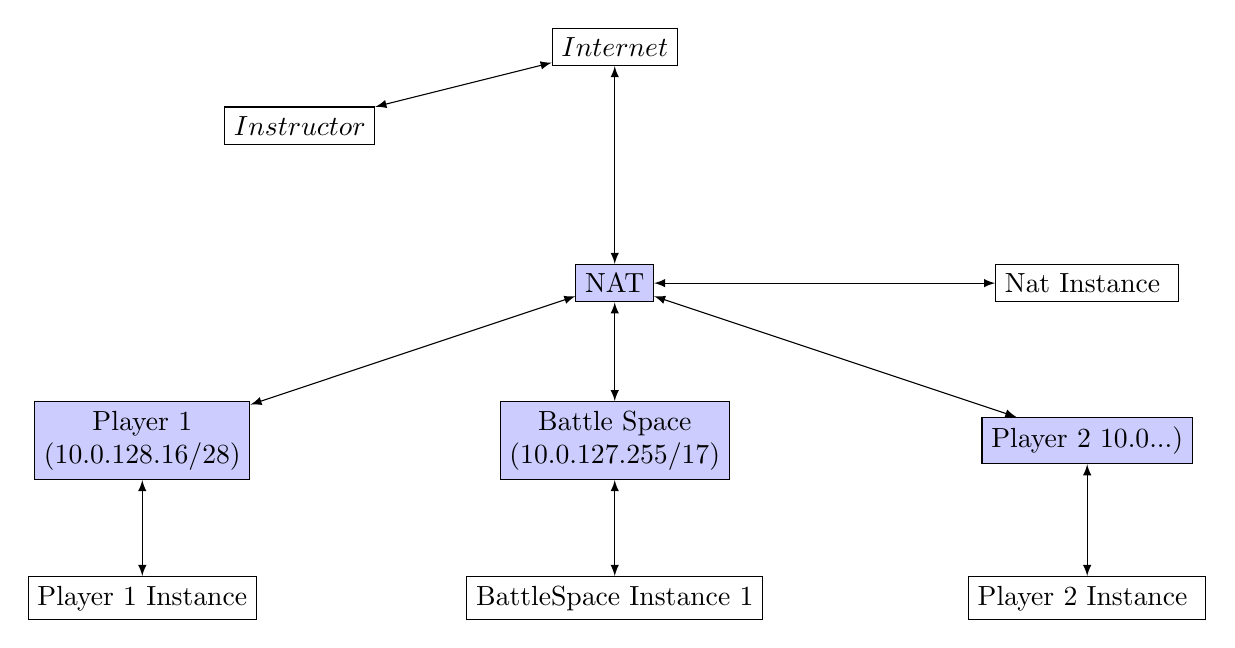
\begin{tikzpicture}[node distance=5mm, >=latex]
%\draw (-1.5,-1) circle (0.5);
   \node (Internet) at (0, 1) [rectangle, draw] {$Internet$};
   \node (Instructor) at (-4, 0) [rectangle, draw] {$Instructor$} edge[<->] (Internet);
   \node (NatSubnet) at (0, -2) [rectangle, subnet, draw] {NAT} edge[<->] (Internet);
   \node (NatInstance) at (6, -2) [rectangle, draw] {Nat Instance } edge[<->] (NatSubnet);

   \node (PlayerTwoSubnet) at (6, -4) [rectangle, subnet, draw] {Player 2 10.0...)} edge[<->] (NatSubnet);
   \node (PlayerTwoInstance) at (6, -6) [rectangle, draw] {Player 2 Instance } edge[<->] (PlayerTwoSubnet);

   \node (PlayerOneSubnet) at (-6, -4) [rectangle, subnet, draw] {Player 1 \\ $(10.0.128.16/28)$} edge[<->] (NatSubnet);
   \node (PlayerOneInstance) at (-6, -6) [rectangle, draw] {Player 1 Instance} edge[<->] (PlayerOneSubnet);

   \node (BattleSpace) at (0, -4) [rectangle, subnet, draw] {Battle Space \\ (10.0.127.255/17)} edge[<->] (NatSubnet);
   \node (BattleSpaceInstance) at (0, -6) [rectangle, draw] {BattleSpace Instance 1} edge[<->] (BattleSpace);

\end{tikzpicture}
\caption{Conceptual diagram of the Recon I game. Note subnets are shaded (blue)}
\end{center}
\end{figure}

There are a dozen hosts on a remote network, and the student tries to find all of them as quickly as 
possible, and discover what what ports are open and what services are running.  At the knowledge level,
the student is learning to use nmap and what options it uses.  At a higher level, the student is learning
about the TCP, UDP and ICMP protocols and how they can be used in ways that may have not been intended.
In more advanced versions, students look for hosts and services that should not be on the network.

EDURange provides the capability to run the same basic scenario, changing the IP addresses and open ports
of the target hosts.  This allows students to repeat the exercise while trying different options of nmap to
find those that meet the goals of a particular variation of the exercise.  For example, the instructor
might ask students to focus on speed or stealth.

\subsubsection{Elf Infection}
Students are given a VM where one of the utilities is infected and listens on a port to open
a reverse shell.  They must figure out which program is infected and what it is doing.
The learning goals are:
\begin{packenum}
\item understand elf format
\item develop the security mindset
\item distinguish between normal and suspicious behavior of programs.
\item use nmap to find hosts and open ports on a network.
\end{packenum}
Concepts from CS 2013 addressed by this module:
\begin{packenum}
\item  risk, threats, vulnerabilities, and attack vectors.  It shows how how an attacker
  could maintain control of a system or exfiltrate data through infected binary files.
\item network security.  The infected software will open a port and send packets to a remote server.
\item trust and trustworthiness.
\item machine-level representation of data
\end{packenum}

\subsubsection{strace}
Students are given a trace of system calls made while a few programs are running simultaneously.
The trace is cleaned up to remove the names of the executable files.
Advanced versions can include malware.

The learning goals are:
\begin{packenum}
\item understand how to sort through complex data
\item develop the security mindset
\item distinguish between normal and suspicious behavior.
\item use strace to characterize aspects of program behavior.
\end{packenum}
Concepts from CS 2013 addressed by this module:
\begin{packenum}
\item  risk, threats, vulnerabilities, and attack vectors.  
\item trust and trustworthiness.
\item digital forensics
\end{packenum}

\subsubsection{scapy hunt}
Students craft network packets to detect hosts that are not visible directly on
the local network.  They observe packets and replaying them with modifications.  They gather
more infromation by overflows the forwarding table and port knocking.

The learning goals are:
\begin{packenum}
\item understand firewall rules
\item develop the security mindset
\item understand routing tables
\item understand how IP works
\end{packenum}
Concepts from CS 2013 addressed by this module:
\begin{packenum}
\item  risk, threats, vulnerabilities, and attack vectors.  
\item network security
\item Access control
\end{packenum}


\subsubsection{Grammar Fuzzing}
This is an attack/defend exercise, where the defender implements a recognizer for a grammar,
e.g. a grammar describing the input to a calculator.  The attacker can look at the code and
 designs input that either creates false postives or false negatives.

The learning goals are:
\begin{packenum}
\item perform input sanitization
\item develop the security mindset
\item understand language security (langsec)~\cite{bratus_SP_2014}
\end{packenum}
Concepts from CS 2013 addressed by this module:
\begin{packenum}
\item  risk, threats, vulnerabilities, and attack vectors.  
\item  language translation
\end{packenum}



\subsection{Addressing CS2013}
Here are the concepts and learning outcomes from CS2013 that we will address:


We will produce additional exercises that will address these goals.

Producing new knowledge about what works effectively.  
In addition to providing a framework for developing exercises at a high level, but we can also 
import VMs that collaborators produce.  We are putting together this service in AWS which we make available
to instructors.  This doesn't use the full power of EDURange, but rather is based on the fact that we
are providing a service through an AWS account where we can make 
The EDURange framework provides an easy way to share exercises.  Every time we have run a workshop, we 
have given surveys and received good suggestions on ways to improve the exercises.


\comment{   a section on current Modules and their structure; this
   foreshadows the Assessment Plan. Modules include: Recon,
   ELFInfection, strace, scapyhunt, calculator grammar fuzzing,

   Description of exericse. analysis skills nurtured, cs 2013 curriculum topic.
   
   List of analysis skills.

   Modules are also an opportunistic mechanism: they provide a
   jumping-off point for discussing a variety of topics mapped to
   a -- exercise motivates each topic discussion or lesson.}
